\documentclass[11pt, a4paper]{article}
\usepackage[utf8]{inputenc}
\usepackage{circuitikz}
\usepackage{siunitx}
\usepackage{amsmath}
\usepackage[italian]{babel}
\usepackage{tablefootnote}
\usepackage{graphicx}
\usepackage{subfigure}
\usepackage{hyperref}

% Table padding
%\renewcommand{\arraystretch}{2}

\ctikzset{
    voltage/bump b=20pt,
    voltage/distance from node=0.5,
    voltage/european label distance=20pt,
}
%\everymath{\displaystyle}
\begin{document}

\title{Teoria dei Sistemi}
\author{Pietro De Nicolao}
\date{\today}
\maketitle

\begin{circuitikz}
\draw(0,0)
to[R, l=$R$, v_>=$v_R$] (0,4)
to[L, l=$L$, v_>=$v_L$, i<=$x_1$, -*] (4,4)
    node[label=A]{}
to[C, l=$C$, v=$x_2$, i>^=$i_C$] (4,0)
to (0,0);
\draw(4,4) to[short, i=$i$] (8,4)
to[generic, l=BNL, v=$x_2$] (8,0)
to (4,0);
\end{circuitikz}

\section*{Dati}
\begin{itemize}
    \item $\alpha = 0.04$
    \item $\beta = 0.18$
    \item $n = 16$
    \item $c = 4$
    \item $L = 12\,\textrm{nH}$
    \item $C = 12\,\textrm{pF}$
\end{itemize}

% -------- PUNTO 1 --------
\section{Equazioni di stato}
Considero l'equazione caratteristica del condensatore $C$:
\begin{equation}
\label{cond-caratt}
i_c = C \dot{x_2}
\end{equation}

Applico LKC al nodo A:
\begin{equation}
i_c = -x_1 - i
\end{equation}

Sostituendo $i_c$ nell'equazione~\ref{cond-caratt}, ottengo la prima equazione di stato:
\begin{equation}
\dot{x_2} = -\frac{1}{C} x_1 + \frac{1}{C}\left( \alpha x_2 - \beta x_2^3\right)
\end{equation}

Poi, considero l'equazione caratteristica del condensatore $L$:
\begin{equation}
\label{ind-caratt}
v_L = L \dot{x_1}
\end{equation}

Applico LKT alla maglia di sinistra, ottenendo:
\begin{equation}
x_2 = v_R + v_L = x_1 R + L \dot{x_1}
\end{equation}

Da cui la seconda equazione di stato:
\begin{equation}
    \dot{x_1} = -\frac{R}{L}x_1 + \frac{1}{L} x_2
\end{equation}

Il sistema è dunque descritto dalle equazioni:
\begin{equation}
    \left\{
    \begin{aligned}
        \dot{x_1} =& -\frac{\strut R}{\strut L}x_1 + \frac{1}{L} x_2\\
        \dot{x_2} =& -\frac{\strut 1}{\strut C} x_1 + \frac{1}{C}\left( \alpha x_2 - \beta x_2^3\right)\\
    \end{aligned}
    \right.
\end{equation}

% -------- PUNTO 2 --------
\section{Assenza di cicli}
L'assenza di cicli per particolari valori di $R$ può essere mostrata grazie al criterio di Bendixon.
\begin{equation}
    \textrm{div f}(x_1, x_2) = \frac{\partial f_1(x_1,x_2)}{\partial x_1} + \frac{\partial f_2(x_1,x_2)}{\partial x_2} = -\frac{R}{L} + \frac{\alpha}{C} - \frac{3\beta}{C}x_2^2
\end{equation}
\begin{equation}\label{big-resistance}
    R > \alpha \frac{L}{C} \Longrightarrow \textrm{div f}<0 \quad \forall x_2
\end{equation}
Per $R > \alpha \frac{L}{C} = 40 \Omega$, la divergenza assume valore negativo per qualunque $x_2$: dunque, non sono presenti cicli nell'intero piano.

Il risultato è in accordo con l'analogia intuitiva che associa la resistenza elettrica con l'attrito nei sistemi meccanici: entrambi i fenomeni dissipano energia e smorzano i movimenti periodici.

% -------- PUNTO 3 --------
\section{Equilibri}
Annullando le derivate delle equazioni del sistema, con semplici passaggi si ricavano le seguenti equazioni:

\begin{equation}
\left\{
\begin{aligned}
    &x_1 ( \beta R^3 x_1^2 - \alpha R + 1) = 0\\
    &x_2 = R x_1\\
\end{aligned}
\right.
\end{equation}

Dunque esiste sempre l'equilibrio banale $x_1 = x_2 = 0$.
Se $R \le \frac{1}{\alpha}$, allora il termine $( \beta R^3 x_1^2 - \alpha R + 1)$ è sempre positivo o nullo e non vi sono altri equilibri.

Altrimenti, esistono altri due equilibri oltre a quello banale.

\begin{table}[h]
\begin{center}
    \begin{tabular}{l | l}
        \textbf{R} & \textbf{Equilibri}\\
        \hline
        $R \le \dfrac{\strut 1}{\strut\alpha}$ & $(0, 0)$\\
        $R > \dfrac{\strut 1}{\strut\alpha}$ & $(0,0),
        \left( \pm \sqrt{\dfrac{\strut\alpha R -1}{\strut\beta R^3}}, \pm \sqrt{\dfrac{\alpha R -1}{\beta R}} \right)$
    \end{tabular}
\end{center}
\caption{Equilibri del sistema al variare di $R$.}
\end{table}

\subsection{Stabilità}
Lo jacobiano del sistema linearizzato è:
\begin{equation}
J(x_1,x_2) =
\begin{bmatrix}
-\dfrac{\strut R}{L\strut} & \dfrac{1}{L} \\
-\dfrac{\strut 1}{C\strut} & \dfrac{\alpha}{C}-\dfrac{\beta}{C} 3x_2^2 \\
\end{bmatrix}
\end{equation}

Analizziamo ora il tipo degli equilibri.
\begin{enumerate}
\item (0,0)\\
\begin{equation}
    J(0,0) =
    \begin{bmatrix}
    -\dfrac{\strut R}{L\strut} & \dfrac{1}{L} \\
    -\dfrac{\strut 1}{C\strut} & \dfrac{\alpha}{C} \\
    \end{bmatrix}
\end{equation}
% Il polinomio caratteristico è nella forma:
% \begin{equation}
%     \lambda^2 + \lambda\left(\frac{R}{L}-\frac{\alpha}{C}\right) + \frac{1-R\alpha}{CL}
% \end{equation}

Calcolo traccia e determinante di $J(0,0)$:
\begin{equation}
\textrm{tr } J(0,0) = \frac{L\alpha-CR}{CL}
\end{equation}
\begin{equation}
\det J(0,0) = \frac{1-r\alpha}{CL}
\end{equation}
L'analisi di stabilità dell'equilibrio è mostrata nella tabella~\ref{stab-00}.

\begin{table}[h]
    \begin{center}
    \begin{tabular}{l l l l l}
        & & tr $J(0,0)$ & $\det J(0,0)$ & tipo\\
        \hline
        $R<\dfrac{1\strut}{\alpha\strut}$ & $(0, 25 \Omega)$ & $>0$ & $>0$ & instabile \\
        \hline
        $\dfrac{1\strut}{\alpha\strut}<R<\dfrac{L\alpha}{C}$ & $(25 \Omega, 40 \Omega)$ & $>0$ & $<0$ & sella \\
        \hline
        $R>\dfrac{L\alpha\strut}{C\strut}$ & $(40 \Omega, +\infty)$ & $<0$ & $<0$ & sella \\
        \hline
    \end{tabular}
    \caption{Stabilità dell'equilibrio $(0,0)$ al variare di R.}
    \label{stab-00}
    \end{center}
\end{table}

\item $\left( \pm \sqrt{\dfrac{\strut\alpha R -1}{\strut\beta R^3}}, \pm \sqrt{\dfrac{\alpha R -1}{\beta R}} \right)$

Questi equilibri esistono solo per $R > \frac{1}{\alpha}$, condizione che dunque può essere assunta nello studio della loro stabilità.

\begin{equation}
    J\left( \pm \sqrt{\dfrac{\strut\alpha R -1}{\strut\beta R^3}}, \pm \sqrt{\dfrac{\alpha R -1}{\beta R}} \right) =
    \begin{bmatrix}
        -\dfrac{R\strut}{L\strut} & \dfrac{1}{L} \\
        -\dfrac{1\strut}{C\strut} & \dfrac{3-2R\alpha}{CR} \\
    \end{bmatrix}
\end{equation}

\begin{equation}
    \det J = 2 \dfrac{R\alpha-1}{CL} > 0 \quad \forall R > \frac{1}{\alpha}
\end{equation}

\begin{equation}
    \textrm{tr } J = \dfrac{-CR^2+3L-2RL\alpha}{CRL}
\end{equation}

\begin{table}[h]
    \begin{center}
    \begin{tabular}{l l l l}
        & tr $J$ & $\det J$ & tipo\\
        \hline
        $\dfrac{1\strut}{\alpha\strut}<R<k$\tablefootnote{$k=\dfrac{-L\alpha + \sqrt{L^2\alpha^2+3LC}}{C} = 27.82 \Omega$}
        & $>0$ & $>0$ & fuoco instabile \\
        \hline
        $R>k$ & $<0$ & $>0$ & fuoco stabile \\
        \hline
    \end{tabular}
    \caption{Stabilità dell'equilibrio $\left( \pm \sqrt{\frac{\alpha R -1}{\beta R^3}}, \pm \sqrt{\frac{\alpha R -1}{\beta R}} \right)$ al variare di R.}
    \label{stab-eq2}
    \end{center}
\end{table}

\subsection{Biforcazioni degli stati di equilibrio}
Per $R=\frac{1}{\alpha}$ l'origine passa da equilibrio instabile a sella, e nascono due nuovi equilibri instabili. Abbiamo dunque una biforcazione forcone, illustrata in \autoref{fig:forcone}.

\begin{figure}
\begin{center}
\subfigure[Biforcazione per $x_1$ al variare di $R$ nell'intorno di $R = 25 \Omega$.]{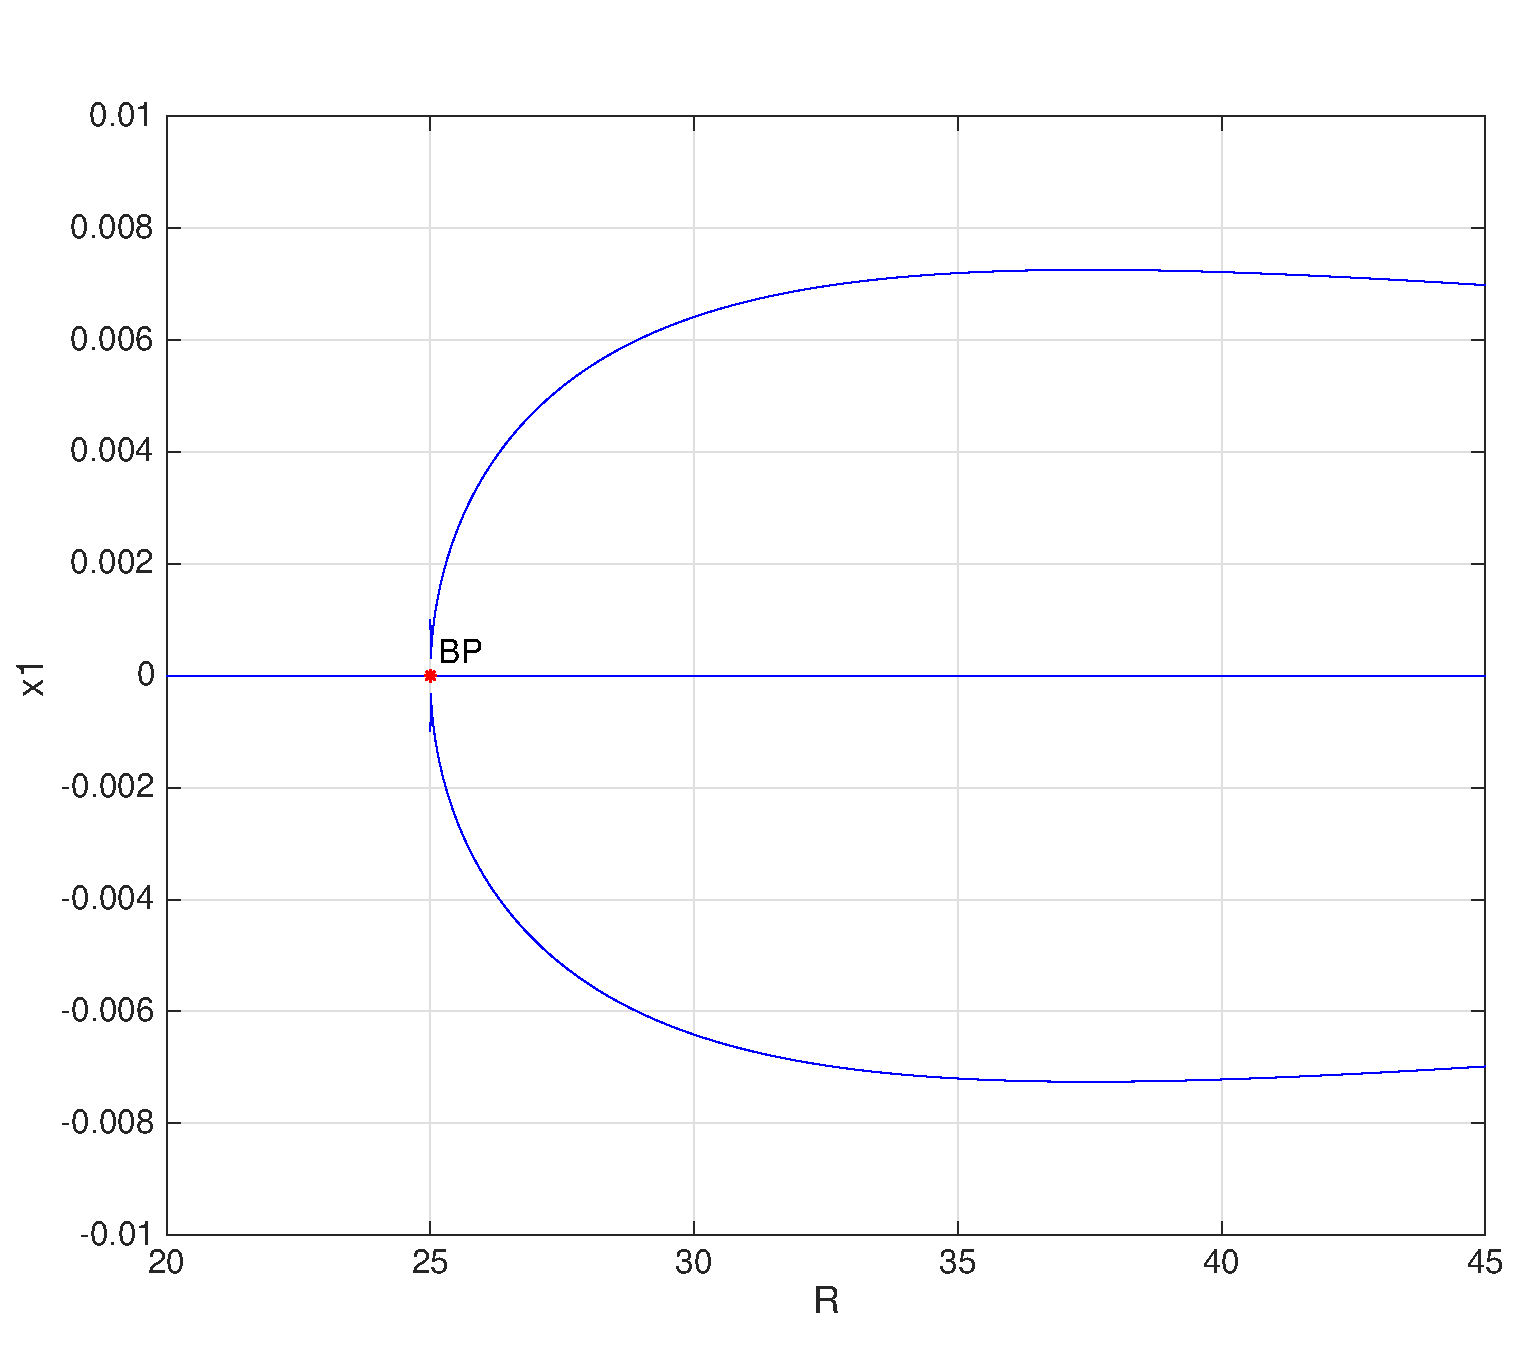
\includegraphics[width=0.8\textwidth]{matcont/BP_25ohm_x1}}
\vfill
\subfigure[Biforcazione per $x_2$ al variare di $R$ nell'intorno di $R = 25 \Omega$.]{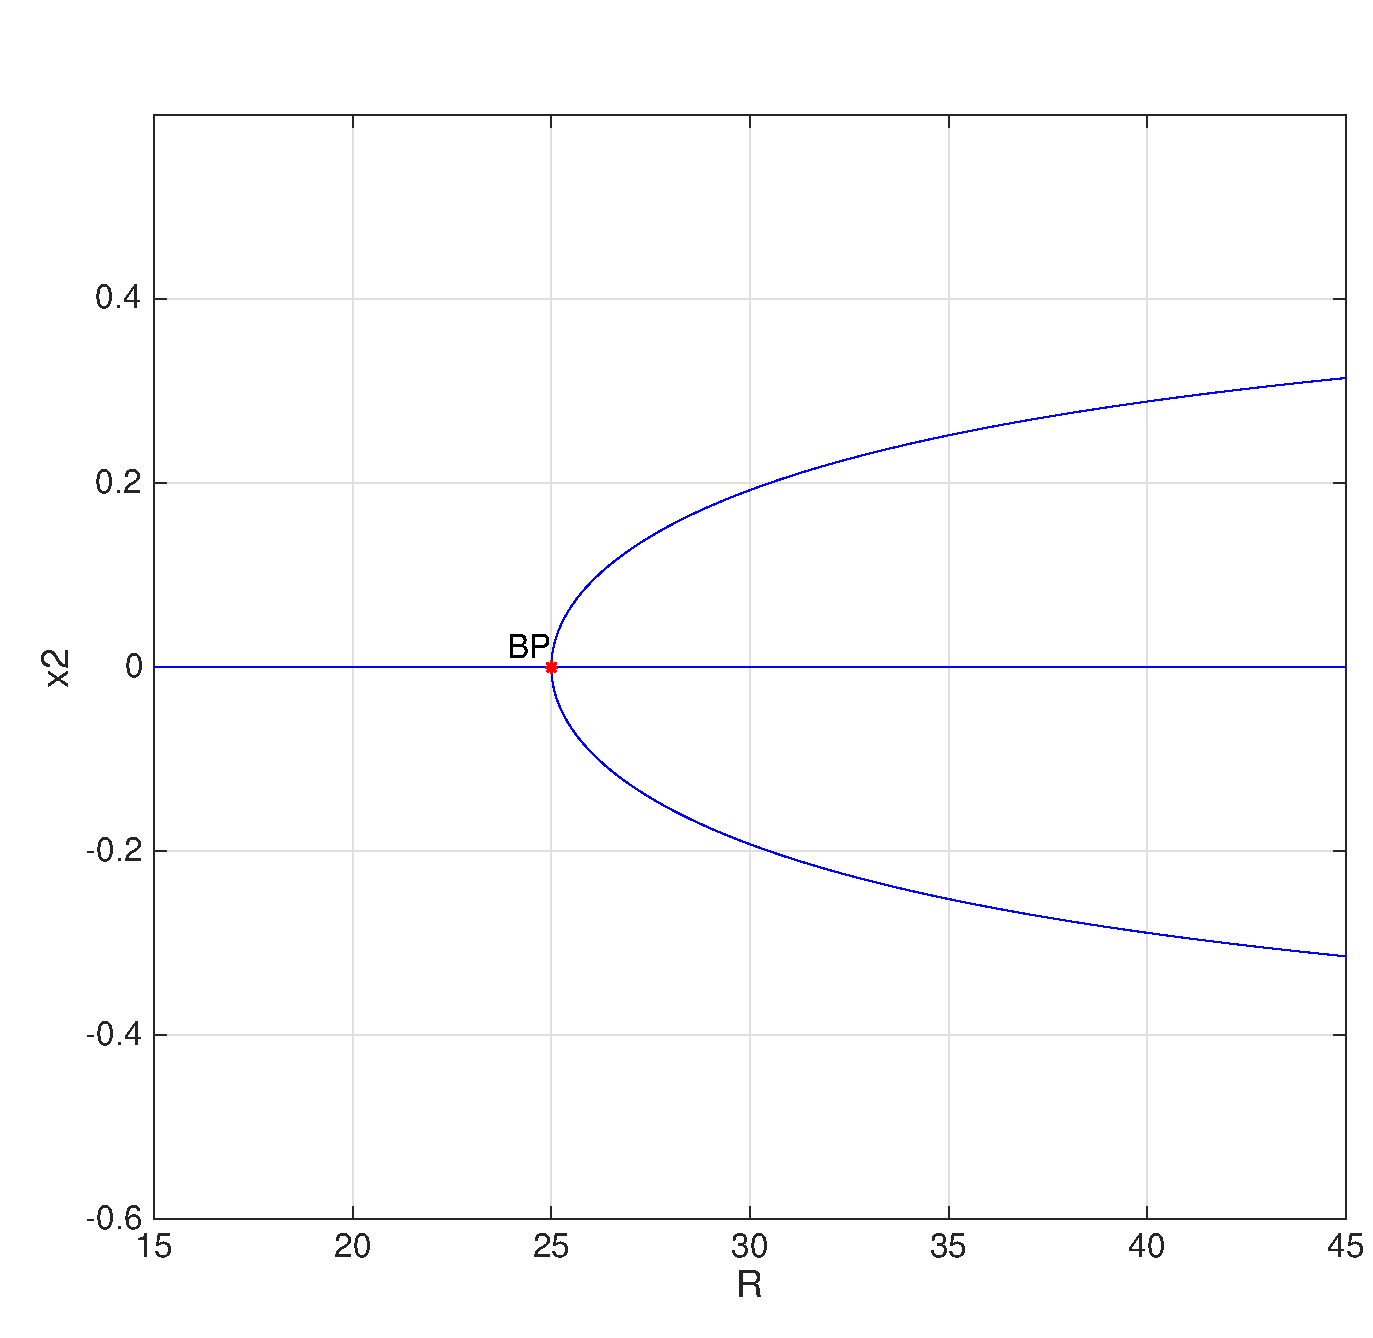
\includegraphics[width=0.8\textwidth]{matcont/BP_25ohm_x2}}
\caption{Biforcazione forcone per $R=25 \Omega$.}
\label{fig:forcone}
\end{center}
\end{figure}

Invece, per $R=k=\dfrac{-L\alpha + \sqrt{L^2\alpha^2+3LC}}{C} = 27.82 \Omega$, i due equilibri diversi dall'origine passano da fuoco instabile a fuoco stabile. La condizione di Hopf è verificata, dunque abbiamo una biforcazione di Hopf supercritica (dalla simulazione, i cicli – stabili – sono dalla parte dell'equilibrio instabile).

\subsection{Cicli}
Per $R<\frac{1}{\alpha}=25 \Omega$, il sistema ammette un ciclo stabile che contiene l'equilibrio instabile.

Per $\frac{1}{\alpha} < R < k$, il sistema ammette un ciclo stabile che contiene l'origine (sella) e i due equilibri instabili, compatibilmente con il criterio di Poincaré.

\begin{figure}
\begin{center}
\subfigure[Ciclo per $R = 15 \Omega$.]{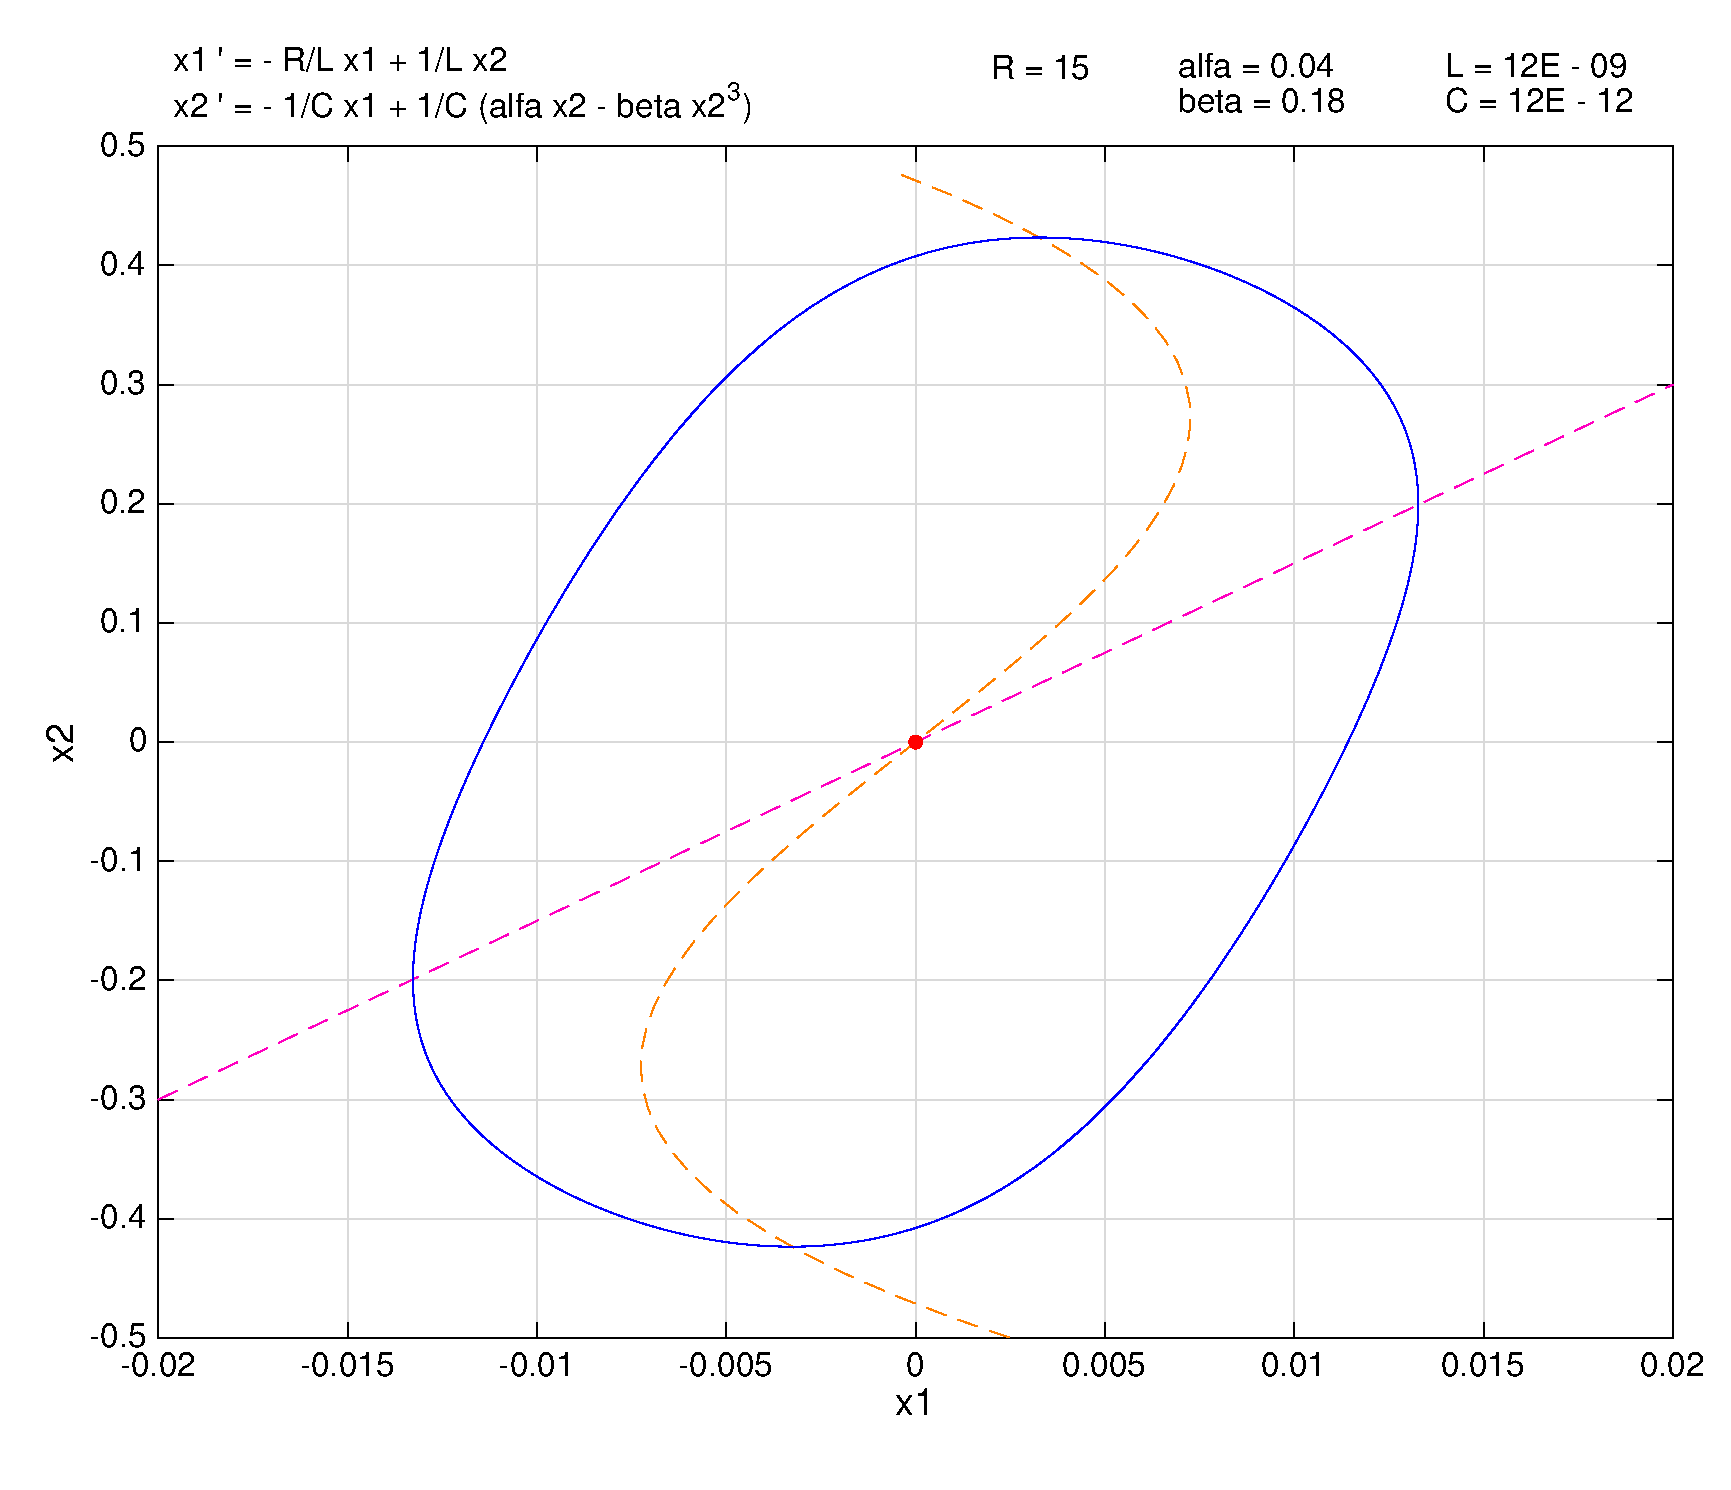
\includegraphics[width=0.8\textwidth]{pplane/Cycle15ohm}}
\vfill
\subfigure[Ciclo per $R = 26 \Omega$.]{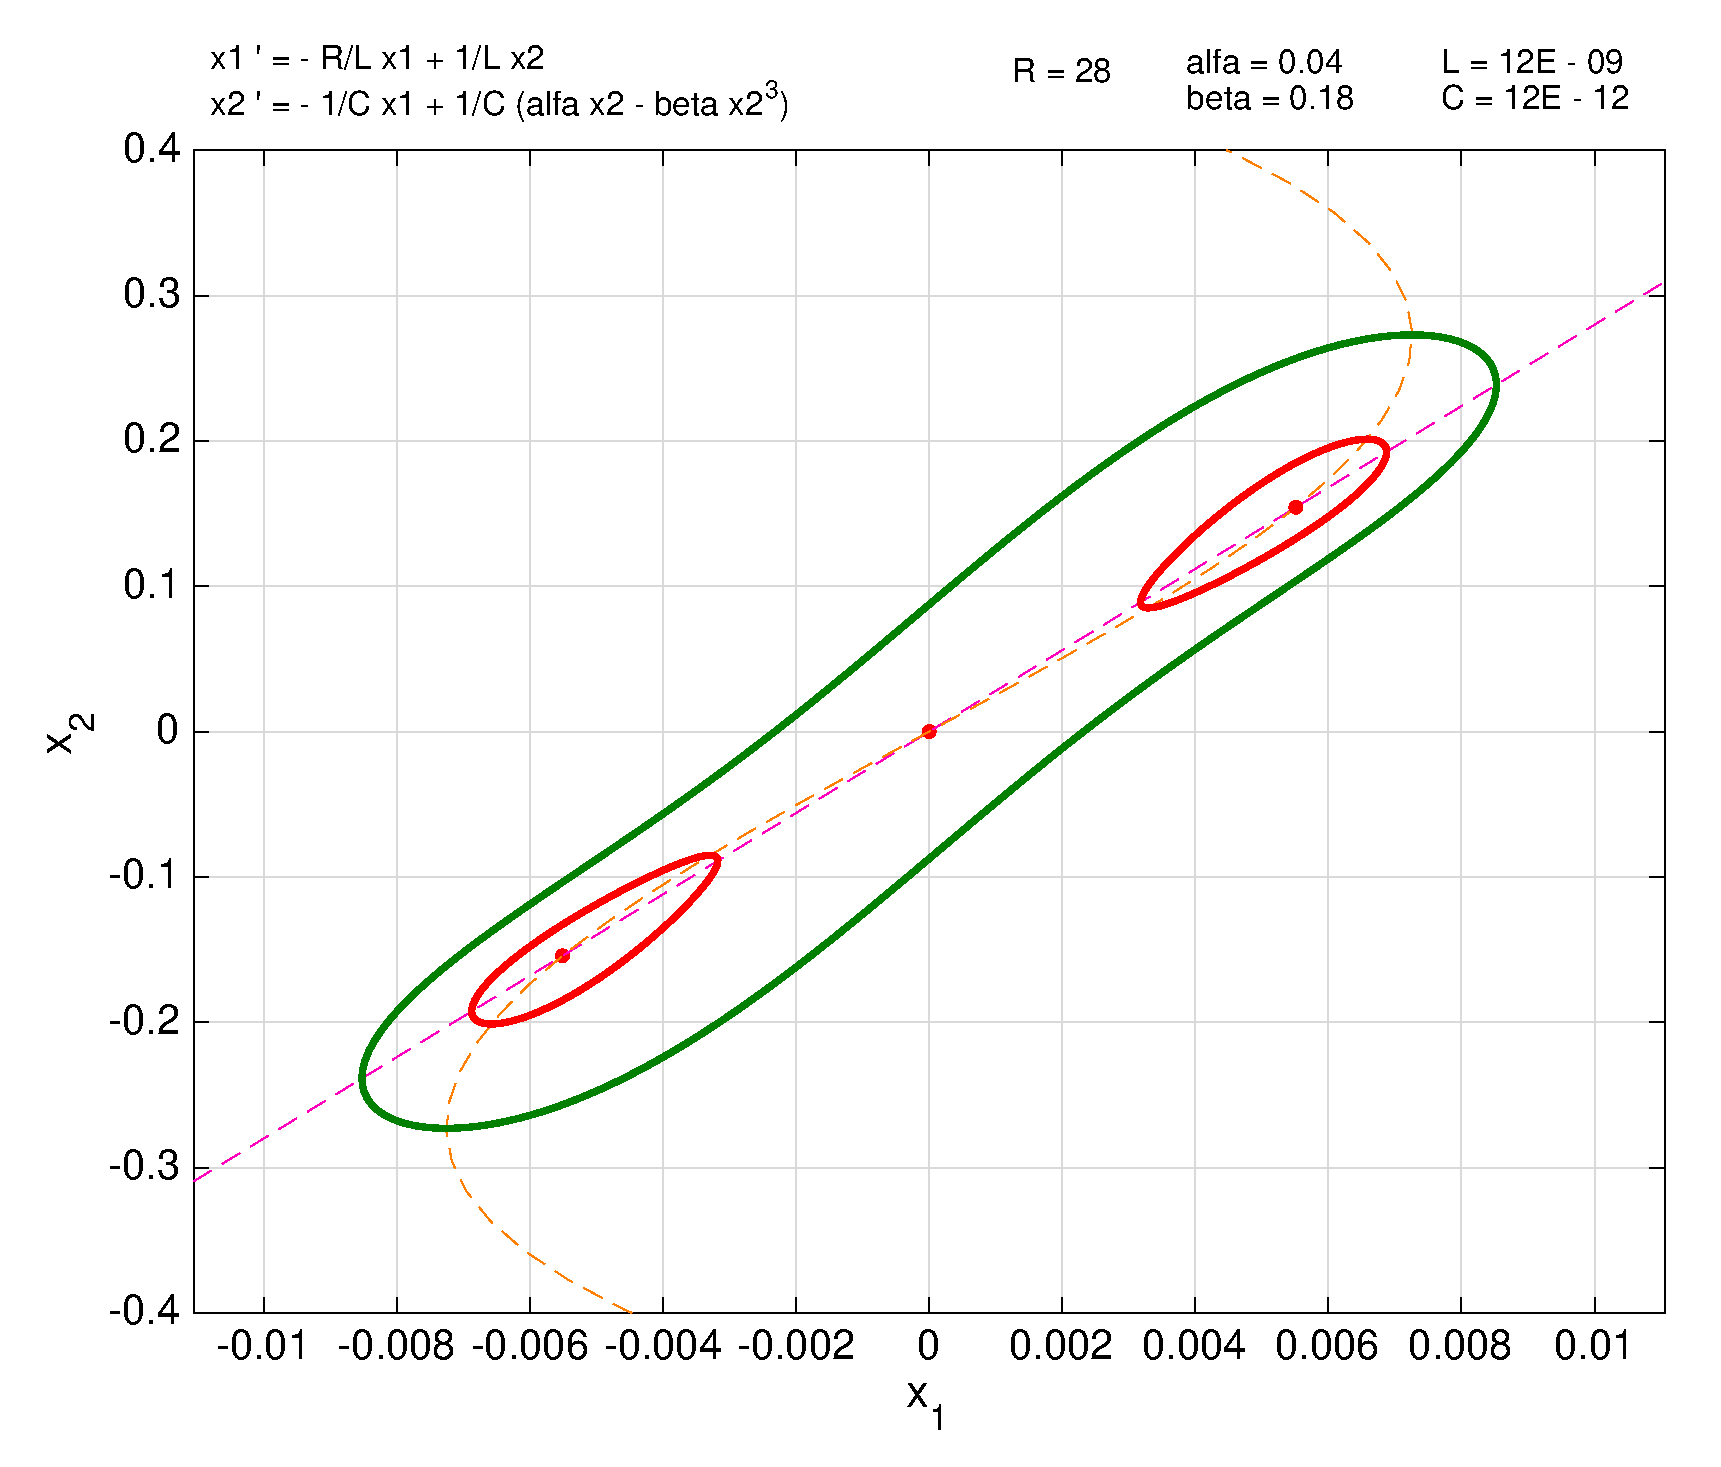
\includegraphics[width=0.8\textwidth]{pplane/Cycle26ohm}}
\caption{Cicli per due parametri di $R$.}
\label{fig:cicli}
\end{center}
\end{figure}

\end{enumerate}
\end{document}
